\documentclass[10pt, hyperref, a4paper]{article}
%\addto\captionsgerman{\renewcommand{\refname}{}}
\usepackage[utf8]{inputenc}
\usepackage[T1]{fontenc}
\usepackage{lmodern}
\usepackage[svgnames]{xcolor}
\usepackage{scrextend} %addmargin functinality

\usepackage[ngerman, english]{babel}
\usepackage[backend=biber, style=ieee, autolang=other]{biblatex}
\bibliography{Literaturverzeichnis} % Link zum Literaturverzeichnis
\usepackage[babel, german=quotes]{csquotes}
\usepackage[font=small,labelfont=bf,textfont=it,
labelsep=endash,margin=10pt,format=plain,labelsep=colon,justification=centerlast,
singlelinecheck=true]{caption}

\usepackage[protrusion=true,expansion=true]{microtype}
\usepackage{amssymb,amsmath,amsfonts}
\usepackage{graphicx}
\usepackage{here}
\usepackage{subfigure}
\usepackage[left=3.25cm,right=3.25cm,top=1cm,bottom=1cm,includeheadfoot]{geometry}
\usepackage{fancyhdr}
\pagestyle{fancy}
\fancyfoot[C]{- \thepage \ -}
\fancyhead[L]{Refactoring Dokumentation}
\fancyhead[R]{FS 2020}
\fancyhead[C]{Übung Multichat}
\renewcommand{\headrulewidth}{0.5pt}
\renewcommand{\footrulewidth}{0.5pt}
\renewcommand{\baselinestretch}{1.2}
\setcounter{tocdepth}{4}
\setcounter{secnumdepth}{4}

\usepackage{epstopdf}
\usepackage{subfig}
\usepackage{booktabs}
\usepackage{fix-cm}
\usepackage{parskip}
\usepackage{url}

\newenvironment{eg} %eingerückt mit Abstandsreduktion
{\vspace{-5pt}
\begin{addmargin}[15pt]{0pt}}
	%bla bla bla
{\end{addmargin}}

\usepackage{array,tabularx}
\newenvironment{conditions}
{\par\vspace{\abovedisplayskip}\noindent
	\tabularx{\columnwidth}{>{$}l<{$} @{}>{${}}c<{{}$}@{} >{\raggedright\arraybackslash}X}}
{\endtabularx\par\vspace{\belowdisplayskip}}



\title{Software-Projekt 2: Übung Multichat\\ \vspace{.7cm}
{\huge Refactoring Dokumentation}}
\date{Abgabe: 17.04.2020}
\author{Autoren: \\Adrian Eyholzer, IT19a, ZHAW SoE, eyholadr@students.zhaw.ch \\Samuel Stalder, IT19a, ZHAW SoE, staldsam@students.zhaw.ch\\\\ Dozent: \\Patrick Feisthammel
\\Dieter Ehrismann
\\Marion Mürner}
\begin{document}
\parindent 0pt
\maketitle

\selectlanguage{ngerman}
\begin{abstract}
Die Hauptaufgabe dieser Übung war das Refactoring der vorgegebenen Multichat Applikation, um ihre Wartbarkeit und Modularität zu verbessern und dadurch weitere Entwicklung zu vereinfachen. Neu dazu kam eine abstrakte Klasse, um Synergien von \texttt{ClientConnectionHandler} und \texttt{ServerConnectionHandler} besser zu nutzen. Die Config-Klasse verbindet in diesem Zusammenhang auch die gemeinsam genutzten Statusdefinitionen. Als letzte zusätzliche Klasse kommt die Data-Klasse. Das Data-Objekt kann auf elegante und saubere Art als Kommunikationsmedium genutzt werden. Fürs Debuggen wurde eine einheitliche Lösung angestrebt. Es wurde im ganzen Projekt ein Logger eingebaut, um global Fehlermeldungen und sonstige Informationen abzufangen. Für die Flexibilität des Programms wurde die Verarbeitung von Daten im Server sowie im Client mit einzelnen Threads ergänzt. Nach den geplanten Änderungen am Source Code wurde erneut eine Codeanalyse durchgeführt. Die erhaltenen Resultate wurden mit dem Anfangszustand verglichen und diskutiert. Der Programmierstil der Applikation wurde aus strukturellen Gründen kaum verändert.
\end{abstract}
\vspace{3.5cm}
\newpage

\tableofcontents

\newpage


\section{Einleitung}
Multichat ist eine Chat-Applikation mit Client- und Servermodul. Die Kommunikation verläuft über ein massgeschneidertes Kommunikations-Protokoll. Die Applikation ermöglicht es mehreren Clients miteinander oder via privater Nachricht (PM) zu kommunizieren. Die Übungsvorgabe umfasst eine Fehlerbehebung sowie ein Refactoring von allen Modulen der Applikation. Beim Refactoring gilt es die interne Struktur des Programmquellcodes zu verbessern, ohne die Funktion zu verändern.\cite{FowlerRuby} Im zweiten Kapitel dieser Dokumentation wird der vorhandene  Quellcode analysiert. Das Ziel ist es hier einen Überblick zu geben. Im dritten Kapitel wird die gewählte Lösung beschrieben. Die vorgenommenen Änderungen an Struktur und Funktionalität werden genauer erläutert. Kapitel \ref{verbesserungen} enthält einige Vorschläge wie das Programm in Zukunft weiter verbessert werden kann. Am Schluss folgt eine Schlussfolgerung der Autoren zur vorliegenden Übung.

\newpage



\section{Resultate unserer Analyse}
Zur Verwendung von Multichat muss zuerst ein Server als verwaltende Instanz gestartet werden; dann können sich Clients verbinden und einander Nachrichten zusenden. Das nachfolgende Kapitel zeigt wie das Programm in seinen Einzelheiten funktioniert und wo Probleme bestehen.

\subsection{Dokumentation der Ursprungsstrukur}

	\begin{figure}[bht!]
		\centering
		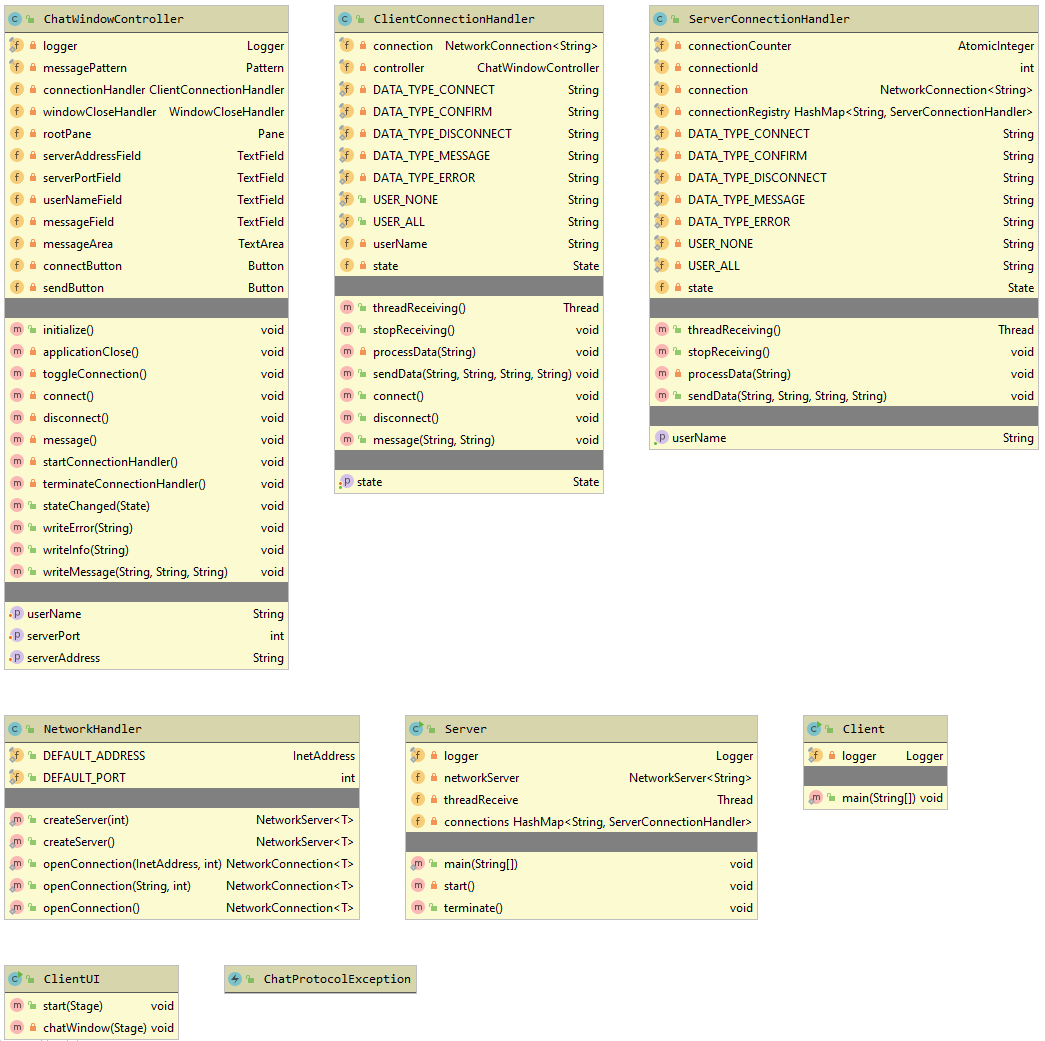
\includegraphics[width=14cm]{..//diagramV1}
		\captionsetup{width=14cm}
		\caption{Klassendiagramm der Applikation nach Erhalt.}
		\label{fig:v1}
	\end{figure}

Abbildung \ref{fig:v1} zeigt die Struktur des Originalprogramms, wobei die Originalmethode «startReceiving» bereits zur neuen Methode «threadReceiving» umbenannt wurde. Die Applikation besteht vor dem Refactoring aus 8 Klassen. Der originale Quellcode von Multichat kann dabei in die Module
\begin{itemize}
	\item Client,
	\item Server,
	\item Protokoll,
\end{itemize}
eingeteilt werden. Es existiert je eine Gradle Konfiguration für den Server- und die Client-Applikation.

Gleicht man das Klassendiagramm mit dem Model-View-Controller Konzept (MVC) ab, stellt man fest, dass dieses Konzept bereits gut umgesetzt ist. \\
Das Model übernimmt der \texttt{ClientConnectionHandler}, Controller ist \texttt{ChatWindowController} und die View läuft über \texttt{ClientGUI}. Alle Interaktionen mit der UI werden vom Controller abgefangen und weitergeleitet. Sämtliche Kommunikation wird im \texttt{ClientConnectionHandler} bearbeitet. Das Model hat keinen direkten Zugriff auf View, was dem Konzept MVC entspricht.

\subsubsection{Bibliotheken}
Multichat verwendet ausser der Java Standard Library und der JavaFX Library keine weiteren Bibliotheken.





\subsection{Dokumentation des Protokolls zwischen Client und Server}

Im Protokoll Modul befinden sich die Klassen \texttt{NetworkHandler}, \texttt{NetworkConnection} und \texttt{NetworkServer}. Die Klasse \texttt{NetworkHandler} wird von den anderen Modulen \texttt{Server} und \texttt{Client} zu Herstellung einer Verbindung, Datenversand und -empfang genutzt (Abb. \ref{fig:protokoll}).\\

	\begin{figure}[bht!]
		\centering
		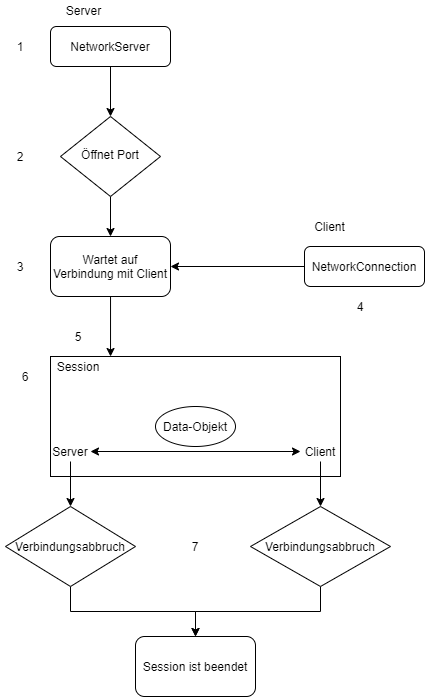
\includegraphics[width=8cm]{..//protokoll.png}
		\captionsetup{width=8cm}
		\caption{Klassendiagramm nach dem Refactoring.}
		\label{fig:protokoll}
	\end{figure}


Beim instanzieren der Klasse \texttt{Server} wird ebenfalls ein neuer Server via \texttt{Networkhandler} gestartet \textbf{(1)}. Dieser erhält den Default-Port 22243 und die IP 0.0.0.0 oder den übergebenen Port-Parameter beim Programmstart \textbf{(2)}. Danach wird der Dienst gestartet und auf dem gewählten Port wird mittels «waitForConnection» auf ein \texttt{NetworkConnection}-Objekt des Clients gewartet \textbf{(3)}. Der Client erstellt nun ein \texttt{NetworkConnection}-Objekt und verbindet sich mit «openConnection» \textbf{(4)}. Der Server erkennt den Verbindungsversuch und erstellt eine Session \textbf{(5)}. In dieser Session können sich Server und Client gegenseitig mittels «receive» und «send» Datenobjekte zuschicken lassen \textbf{(6)}. Das Datenobjekt besteht aus den vier Komponenten Sender, Receiver, Type und Payload. Sender und Receiver beinhalten einen bestimmten User. Mit «*» kann ein Sender eine Nachricht an alle Empfänger schickten. Der Type vermittelt, zu welchem Zweck die Daten verschickt wurden und im Payload ist die eigentliche Nachricht enthalten. Sobald entweder der Client oder der Server mittels «close» die Verbindung unterbricht, terminiert die Session und die Kommunikation zerfällt \textbf{(7)}.\\
Eine Gefahrenquelle ist hier das gleichzeitige Verarbeiten und Senden von Datenobjekten. Dies kann ohne separaten Thread nicht gewährleistet werden.





\subsection{Beschreibung der gefundenen funktionalen Fehler}\label{funk}

\subsubsection{\texttt{Client} kann keine Daten verarbeiten}
Ein Herstellen der Verbindung zwischen Client und Server gelingt zuerst nicht. Es scheint, als ob der Client blockiert, denn seine Weiterverwendung ist unmöglich. Eine erste Vermutung ist, dass der Server in einen Dead-Lock läuft oder die Anfrage nicht bearbeiten kann. Nach einigem Nachforschen war klar, dass das Problem beim Client liegt. Er kann Daten nicht gleichzeitig empfangen und verarbeiten. Die Methode «startReceiving» im Client blockierte die Frontend-Anwendung. Das Problem liegt also nicht an der Verbindung zwischen Client und Server, sondern bei der Implementierung der Datenverarbeitung.

\subsubsection{\texttt{Server} kann nur einen Client betreuen}
Ein weiteres Problem besteht beim Servermodul. Der Server kann nur einen Client betreuen. Dies liegt daran, dass die Methode «startReceive» nur einmal ausgeführt werden kann. Es existiert keine Möglichkeit mehrere Clientverbindungen nebeneinander laufen zu lassen.

\subsubsection{Inputverifikation}
Der \texttt{ChatWindowController} lässt im Client falschen Userinput für die Felder \texttt{UserName}, \texttt{Port} und \texttt{IP-Adresse} zu. 




\subsection{Beschreibung der gefundenen strukturellen Fehler}\label{struk}
Programme können auf unterschiedlichste Weise programmiert sein und trotzdem dieselben Aufgaben erfüllen. Ist dieser Code unzureichend dokumentiert, wird es schwierig vorhandenen Code zu warten oder zu optimieren. Eine Methode muss genau das erledigen, was in ihrer Dokumentation steht. Code soll nach gängigen Prinzipien verfasst und formatiert werden. Solche Regeln vereinfachen das Zusammenarbeiten und Kommunizieren bei der Entwicklung und bei der Wartung. In der Applikation Multichat haben wir auf grundlegende strukturelle Fehler geachtet. Diese Fehler werden üblicherweise \emph{Code Smells} genannt.\cite{Fowler1999} Ein Refactoring von solchen schlechten Programmteilen führt oft zu einer erheblichen Qualitätsverbesserung des vorliegenden Codes. Nachfolgend werden Code Layout und Klassendiagramm genauer untersucht.

\subsubsection{Code Layout} \label{smells}
Die Code-Einrückung und Einteilung des Codes in Blöcke, wurden nur stellenweise umgesetzt. Toter Code und sehr lange Codezeilen, sowie lange Methoden wurde gefunden. Der Code enthielt ausserdem Magic Numbers; passende Namen für Booleans fehlten. Javadoc fehlt teilweise.

\subsubsection{Klassendiagramm/Codeduplikate}
In den Klassen \texttt{ServerConnectionHandler} und \texttt{ClientConnectionHandler} gibt es viele ähnliche Methoden davon sind die Methoden «stopReceiving» und «processData» identisch. Diesen Code kann man in eine abstrakte Superklasse auslagern. Ausserdem sind viele Enums und statische Variablen gemeinsam genutzt. Auch hier wäre eine Auslagerung in eine Config-Klasse sinnvoll.

\subsubsection{Statusmeldung/Logging}
Ausser in den Klassen \texttt{Client} und \texttt{Server} werden alle Statusmeldung über \texttt{System.out.err} an die Clientoberfläche übergeben. Dies könnte durch Ausweitung des bereits stellenweise implementierten Loggers erreicht werden.




\section{Beschreibung unserer Lösung}

\subsection{Funktionale Änderungen}
Die Überarbeitung der Punkte aus Kapitel \ref{funk} sind essenziell für die korrekte Programmfunktionalität. Nachfolgend wird kurz für jedes Problem eine Lösung präsentiert. 

\subsubsection{\texttt{Client} kann keine Daten verarbeiten}
Das Problem wurde gelöst, indem die receive-Methode des Clients in einen Thread gelegt wurde. Für die Verwaltung des Threads wurde der \texttt{ExecutorService} verwendet. Im Client wird ein \texttt{SingleThreadExecutor} verwendet, weil immer nur ein Thread benötigt wird. Dieser wird beim Verbinden erzeugt und beim Trennen gelöscht. 

\subsubsection{\texttt{Server} kann nur einen Client betreuen}
Zur Betreuung von mehreren Clients wurde die receive-Methode des Backends ebenfalls in einen Thread gelegt. Genauer wurde beim Server ein \texttt{FixedThreadPool} verwendet. Für den Server wurden 8 Threads definiert, das heisst es werden 8 Clients gleichzeitig unterstützt. Wir haben uns für eine fixe Zahl entschieden um den Server für eine kleine Gruppe optimal laufenzulassen. Es sind somit Gruppen von 2-8 Personen möglich.

\subsubsection{Inputverifikation}
Für die betroffenen Felder \texttt{UserName}, \texttt{Port} und \texttt{IP-Adresse} wurden mit Regex-Pattern gearbeitet. Falscher Input wird nun verifiziert und falls nötig werden Hinweismeldungen ausgegeben.


\subsection{Strukturelle Änderungen}
Grundsätzlich dienen alle Änderungen des Codelayouts einer besseren Übersicht und Lesbarkeit des Codes. Nachfolgend werden die Vorteile der in \ref{struk} erwähnten Punkte kurz erläutert.

\subsubsection{Code Layout}
In unserem Refactoring haben wir strukturell einige Änderungen vorgenommen. Zum einen haben wir die \emph{Code smells} aus Kapitel \ref{smells} entfernt. Das heisst, es wurden Bereiche ohne Klammern mit Klammern versehen, falsche Code-Einrückung korrigiert. Nicht verwendete Konstruktoren in der Klasse \texttt{ChatProtocolException} wurden entfernt. Magic Numbers wurden zu statischen Variablen umgewandelt. Booleans wurden mit passenden Namen versehen. Zum Schluss wurde der gesamte public Code mit Javadoc versehen. 
%klassen alle italic
\subsubsection{Codeduplikate und Datenobjekt}
Gefundenen Codeduplikate wurden entfernt beziehungsweise ausgelagert. Die beiden identischen Methoden aus \texttt{ClientConnectionHandler} und \texttt{ServerConnectionHandler} wurden in eine abstrakte Superklasse \texttt{ConnectionHandler} ausgelagert.\\
Ausserdem wurde das versendete Paket, welches aus mehreren Strings besteht, in ein neues Datenobjekt \texttt{Data} ausgelagert.

\subsubsection{Logging}
Der bereits implementierte Java-Logger wurde flächendeckend implementiert und mit ersten Logger-Leveln versehen. Sämtliche Ausgaben via \texttt{System.out.err} wurden ersetzt.






\subsection{Dokumentation der Struktur nach dem Refactoring}
Abbildung \ref{fig:v3} zeigt die neue Projektstruktur. Sie enthält zwei neue Klassen: eine Klasse für das neue eingeführte \texttt{Data}-Objekt und eine abstrakte Klasse \texttt{ConnectionHandler}.

	\begin{figure}[bht!]
		\centering
		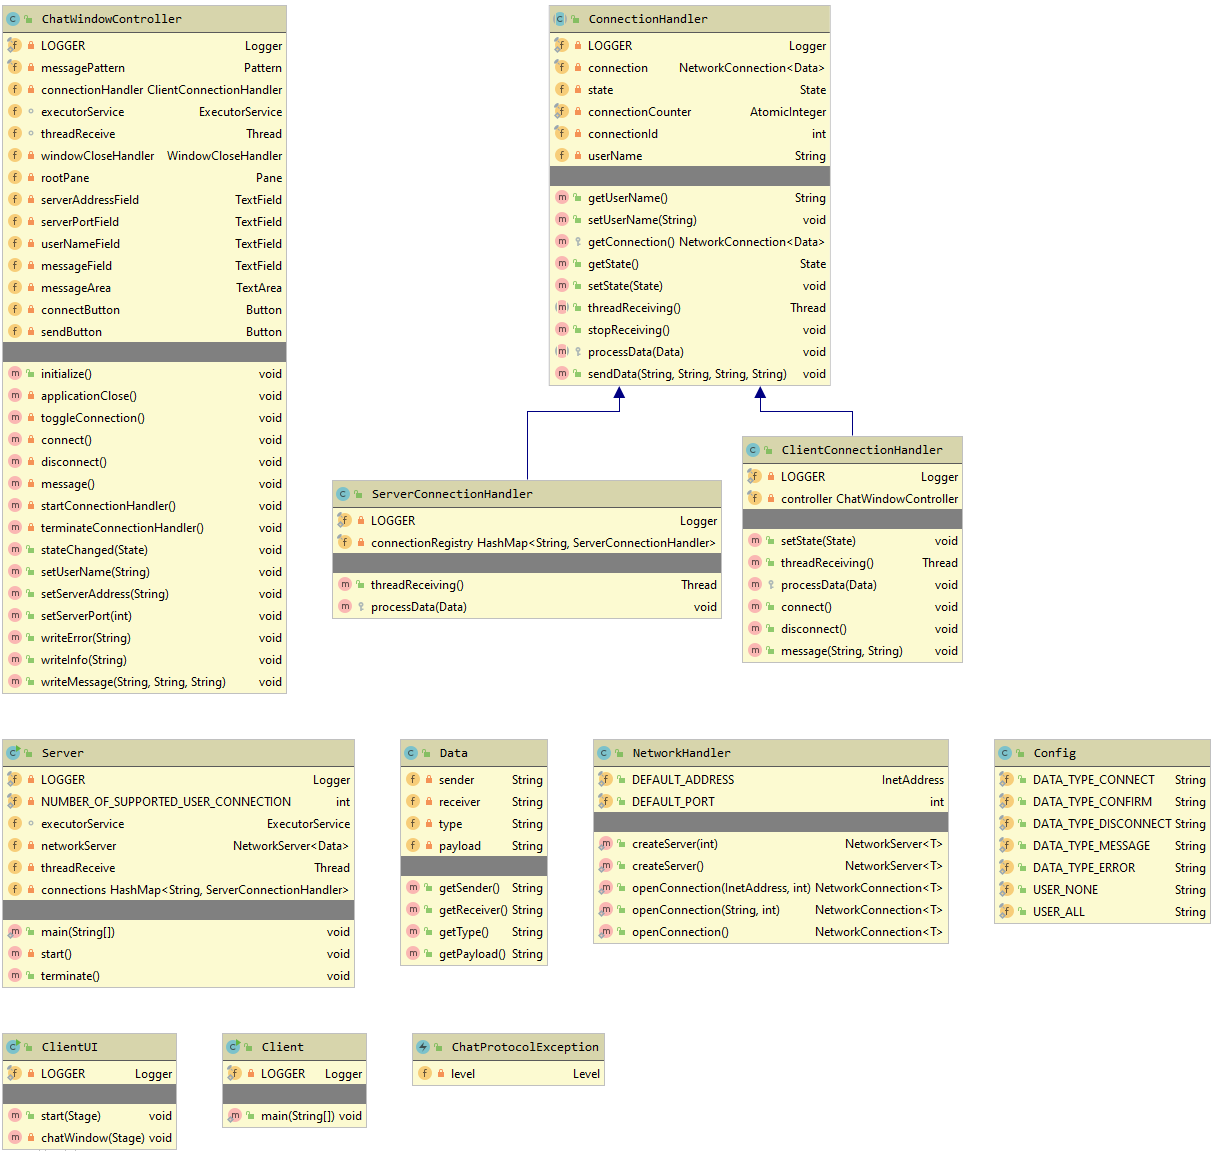
\includegraphics[width=14cm]{..//diagramV3}
		\captionsetup{width=14cm}
		\caption{Klassendiagramm nach dem Refactoring.}
		\label{fig:v3}
	\end{figure}





\subsection{Erläuterungen zur Lösung der vorliegenden Probleme}
In diesem Teil werden die Vorteile unserer gewählten Lösung besprochen. Zu jedem oben erwähnten Problem folgt eine kurze Analyse.

\subsubsection{\texttt{Client} kann keine Daten verarbeiten}
Der Einsatz eines \texttt{SingleThreadExecutor} ist hier sinnvoll, weil jeder Client nur einen Thread für den Datenempfang benötigt. Der Einsatz des \texttt{ExecutorServices} ermöglicht ausserdem ein einfaches Erstellen und Beenden des Thread beim Verbinden bzw. Trennen.

\subsubsection{\texttt{Server} kann nur einen Client betreuen}
Durch die Verwendung eines \texttt{FixedThreadPool} kann die Anzahl der gleichzeitigen Clientverbindungen einfach gesteuert werden. Um das Verhalten des Serversystems bei mehr als 8 Clients abschätzen zu können, wären Hardwareanforderungstests sinnvoll. Nur so kann ein problemloser Langzeitbetrieb mit mehr als 8 Clients garantiert werden. 

\subsubsection{Inputverifikation}
Durch die Verwendung von Regex-Pattern kann der Userinput sehr genau eingeschränkt und so verifiziert werden. Die Lösung ist schlank und unkompliziert.

\subsubsection{Code Layout}
In unserem Refactoring haben wir durch korrekte Klammersetzung und Einrückung die Anzahl Codezeilen verringert und die Leserlichkeit verbessert.
Namen von Booleans wurden nach ihrem assoziierten Fall gewählt, Magic Numbers wurden durch statische Variablen ersetzt. Beides macht den Code selbsterklärender und leichter lesbar wurde.

\subsubsection{Spekulative Implementationen}
Die zwei Konstruktoren der \texttt{ChatProtocolException} Klasse, welche für zukünftige Funktionalitäten vorgesehen sind jedoch nie richtig ins Programm eingebunden wurden, wurden entfernt. Methoden, welche erst in zukünftige Funktionalitäten benötigt werden, sollten grundsätzlich erst eingebunden werden, sobald die Funktionalität benötigt wird.

\subsubsection{Dokumentation}
Im ganzen Projekt wurde Javadoc eingefügt, dies ist sehr wichtig für die Betreuung und Weiterentwicklung der Software. Ohne Erklärung was ein Code machen soll, bleibt dem Betreuer nichts anderes übrig als abhängig vom vorhandenen Code zu entscheiden, ob die gewünschte Funktion vorliegt. Dies gilt es zu verhindern.

\subsubsection{Datenobjekt \texttt{Data}}
Wenn Daten an einem Ort im Code vermehrt zusammen auftreten, ist es sinnvoll diese in eine neue Klasse bzw. Objekt zu extrahieren. Mittels Stringbuilder wurde im alten Code aus einzelnen Strings der Datenstring zusammengebaut. Das neu eingeführte Datenobjekt \texttt{Data} ersetzt die Stringbuilderaktion und macht den Code übersichtlicher und leichter verwendbar.

\subsubsection{Codeduplikate}
Codeduplikate weisen auf ein Design ohne ausreichende Abstraktion hin. Sie verringern die Übersichtlichkeit und Wartbarkeit von Code, da Änderungen an mehreren Stellen vorgenommen werden müssen.\\
Mit dem Entfernen von Codeduplikaten kann sehr einfach die Masse des Codes reduziert werden, ohne aber seine Funktionalität zu verlieren. Es wird empfohlen Codeduplikate in eine Methode auszulagern \cite{Fowler1999} - was beim Refacotring auch so umgesetzt wurde.

\subsubsection{Allgemeine Einschätzung}
Unsere Änderungen sind bezogen auf die investierte Zeit optimal. Unser simples Chatprogramm funktioniert wie gewünscht, alle Funktionalitäten sind vorhanden. Die Optimierung von Struktur (Datenobjekt, abstrakte Klasse) und Layout helfen dem betreuenden Programmierer in Zukunft zeitnah neue Features zu implementieren und allfällige Bugs mit dem optimierten Logger-Tree zu bearbeiten. Durch die Reduktion der Code-Komplexität wurde die Wartbarkeit erhöht und die zukünftige Arbeitseffizienz verbessert.





\section{Zukünftige Verbesserungsmöglichkeiten} \label{verbesserungen}
Da der Faktor Zeit bei dieser Übung eine grosse Rolle gespielt hat, schlagen wir nachfolgend noch einige Modifikationen vor, welche in Zukunft als erstes bearbeitet werden sollten.\\
Es ist unumgänglich detailliert Tests für Multichat zu schreiben, nur so kann zukünftige Entwicklung effizient vorangetrieben werden. Dies zieht auch ein Anpassen der Logger-Level auf die Tests mit sich. Ausserdem würde ein kürzen einiger Methoden, vorallem der main-Methoden sinnvoll sein. Die \texttt{NetworkHandler}-Klasse war gemäss Vorgabe nicht zu optimieren; dennoch wäre ein Extrahieren der darin enthaltenen Subklassen \texttt{NetworkConnection} und \texttt{NetworkServer} in eigene Klassen sehr sinnvoll. Je länger Klassen und Methoden sind, desto schwieriger ist es deren Funktion zu verstehen. Verbesserungspotential birgt auch die Fehlerrückgabe. Momentan werden diese unstrukturiert in der Text-Area angezeigt. An dieser Stelle wären Alerts oder andere Warnmeldungen visuell ansprechender. Ein etwas grösserer Aufwand wäre die Erweiterung der Reichweite. Im aktuellen Projekt kann nur im lokalen Netzwerk kommuniziert werden. Man könnte einen öffentlich zugänglichen Server mit fixer IP-Adresse einrichten, um mehr Kommunikationsfreiheiten zu ermöglichen. 



\section{Schlussfolgerung}
Mit dem Abschluss dieses Projekts durften wir einige neue Sachen Lernen und viel Gelerntes festigen. Im Grossen und Ganzen hat uns dieses Projekt sowie die bisherigen Projekte gut gefallen. Die Aufgabenstellung war gut dokumentiert und die Lehrpersonen standen uns für Fragen immer zur Seite. Das Thema war spannend und gut abgesprochen mit «Programmieren 2». Wir freuen uns bereits auf die nächste Teamarbeit.



\printbibliography[heading=bibnumbered,title={Literaturverzeichnis}]


\end{document}
